
\documentclass[11pt,a4paper]{article}

\usepackage[margin=1in]{geometry}
\usepackage[T1]{fontenc}
\usepackage[utf8]{inputenc}
\usepackage{lmodern}
\usepackage{microtype}
\usepackage{xcolor}
\usepackage{booktabs}
\usepackage{longtable}
\usepackage{array}
\usepackage{enumitem}
\usepackage{hyperref}


\usepackage{tikz}
\usetikzlibrary{arrows.meta,positioning,fit,calc,shapes.geometric,backgrounds}
\usepackage{float}

\definecolor{navy}{RGB}{28,54,92}
\definecolor{blue2}{RGB}{62,112,170}
\definecolor{lightblue}{RGB}{232,242,252}
\definecolor{green2}{RGB}{50,120,80}
\definecolor{lightgreen}{RGB}{235,247,239}
\definecolor{orange2}{RGB}{190,105,25}
\definecolor{lightorange}{RGB}{252,243,229}
\definecolor{red2}{RGB}{170,55,55}
\definecolor{lightred}{RGB}{252,237,237}

\tikzset{
  agentbox/.style={draw=blue2, rounded corners=4pt, thick,
    minimum width=30mm, minimum height=11mm, align=center, fill=lightblue},
  toolbox/.style={draw=green2, rounded corners=4pt, thick,
    minimum width=30mm, minimum height=11mm, align=center, fill=lightgreen},
  databox/.style={draw=orange2, rounded corners=4pt, thick,
    minimum width=32mm, minimum height=11mm, align=center, fill=lightorange},
  securitybox/.style={draw=red2, rounded corners=4pt, thick,
    minimum width=30mm, minimum height=11mm, align=center, fill=lightred},
  flow/.style={-{Latex[length=2mm]}, thick},
  dashedflow/.style={-{Latex[length=2mm]}, thick, dashed},
  decision/.style={diamond, draw=navy, thick, aspect=2, align=center, fill=white}
}

\usetikzlibrary{arrows.meta,positioning,fit,calc,shapes.geometric}
\usepackage{listings}
\usepackage{amsmath}
\usepackage{fancyhdr}

\definecolor{navy}{RGB}{30,55,90}
\definecolor{lightblue}{RGB}{235,243,252}
\definecolor{lightgray}{RGB}{245,245,245}
\definecolor{darkgray}{RGB}{80,80,80}

\hypersetup{
    colorlinks=true,
    linkcolor=navy,
    urlcolor=navy,
    pdftitle={Multi-Agent Database Analyzer and Agentic Chat Support},
    pdfauthor={Student Handout}
}

\pagestyle{fancy}
\fancyhf{}
\lhead{Multi-Agent Database Analyzer}
\rhead{sujeet.banerjee@gmail.com \\
sujeet.banerjee.professional@gmail.com}
\cfoot{\thepage}

\lstset{
    basicstyle=\ttfamily\small,
    backgroundcolor=\color{lightgray},
    frame=single,
    breaklines=true,
    columns=fullflexible
}

\newcommand{\agent}[1]{\textbf{\textcolor{navy}{#1}}}
\newcommand{\important}[1]{\textbf{#1}}

\title{\textbf{Multi-Agent Database Analyzer}\\
\large Architecture, System Design and Agentic Chat Support}
\author{Sujeet Banerjee}
\date{}

\begin{document}
\maketitle

\begin{description}
 
This handout presents the architecture and system design of a multi-agent
Database Analyzer that allows users to ask natural-language questions about
large databases and receive evidence-based summaries, analysis, and
follow-up insights. The system combines agentic orchestration, schema and
metadata retrieval, Text-to-SQL, query validation, database-side computation,
statistical analysis, and an LLM-based conversational interface.

A central design principle is that the LLM should not attempt to ingest an
entire database. Instead, the database performs the heavy computation and the
agents coordinate what should be queried, analyzed, and investigated. This
architecture makes the approach more scalable, safer, and more auditable.
\end{description}


\section*{Architecture at a Glance}
\addcontentsline{toc}{section}{Architecture at a Glance}

\begin{figure}[H]
\centering
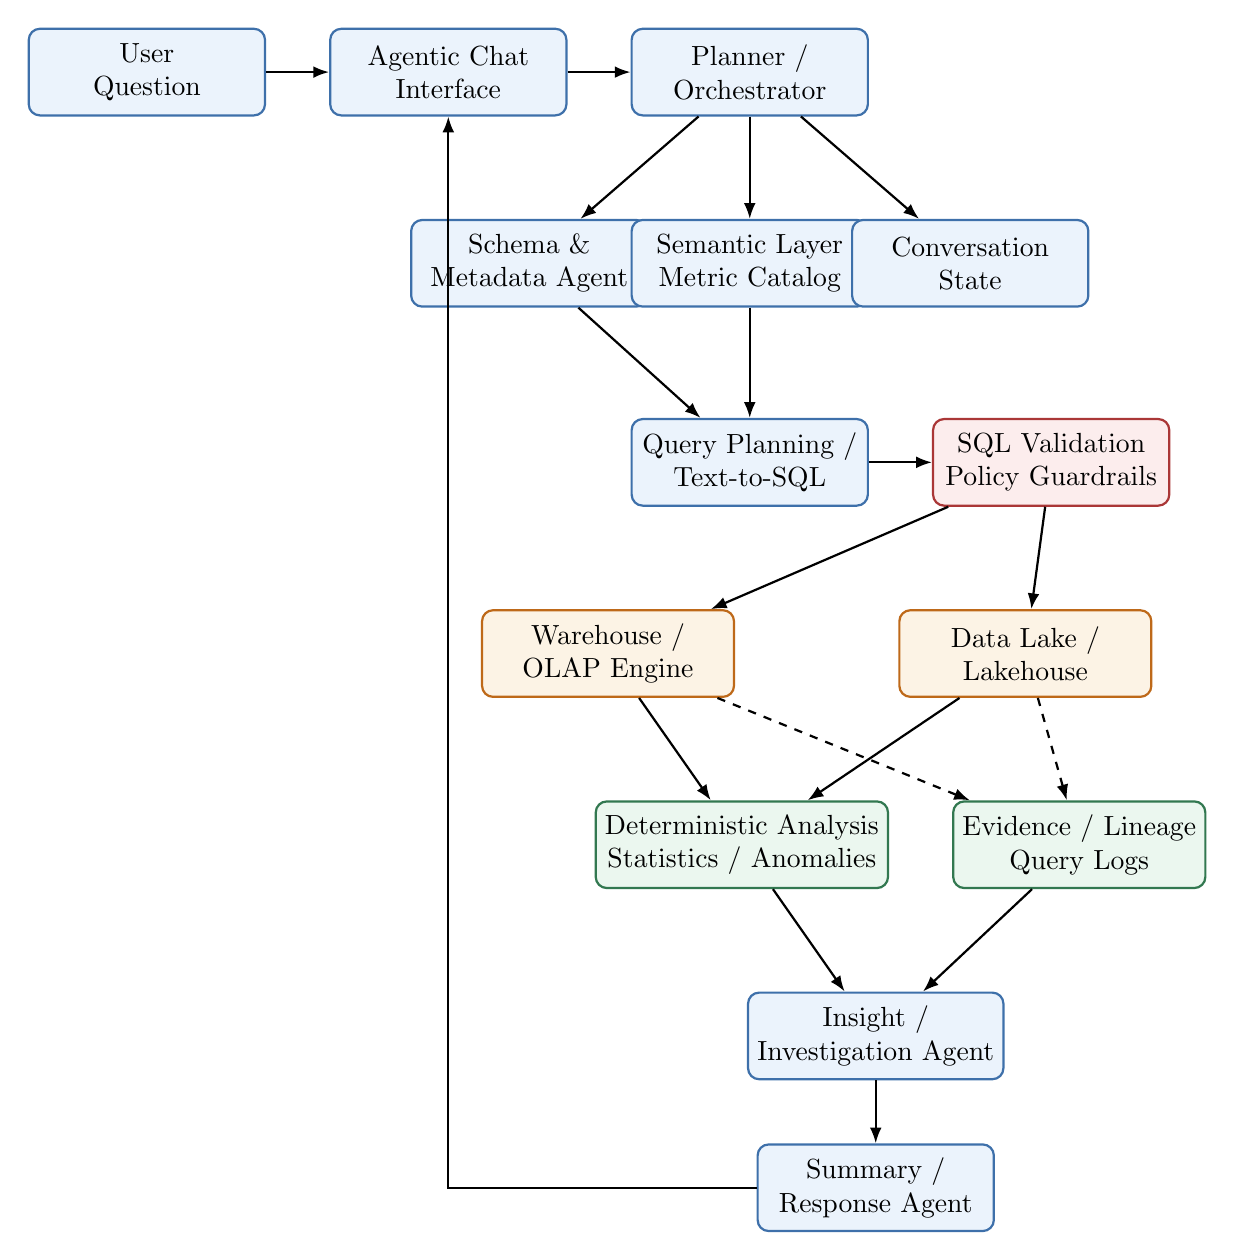
\begin{tikzpicture}[node distance=8mm and 8mm]
\node[agentbox] (user) {User\\Question};
\node[agentbox, right=of user] (chat) {Agentic Chat\\Interface};
\node[agentbox, right=of chat] (planner) {Planner /\\Orchestrator};

\node[agentbox, below=13mm of planner, xshift=-28mm] (schema)
{Schema \&\\Metadata Agent};
\node[agentbox, below=13mm of planner] (semantic)
{Semantic Layer\\Metric Catalog};
\node[agentbox, below=13mm of planner, xshift=28mm] (memory)
{Conversation\\State};

\node[agentbox, below=14mm of semantic] (query)
{Query Planning /\\Text-to-SQL};
\node[securitybox, right=of query] (guard)
{SQL Validation\\Policy Guardrails};

\node[databox, below=13mm of query, xshift=-18mm] (warehouse)
{Warehouse /\\OLAP Engine};
\node[databox, below=13mm of query, xshift=35mm] (lake)
{Data Lake /\\Lakehouse};

\node[toolbox, below=13mm of warehouse, xshift=17mm] (analysis)
{Deterministic Analysis\\Statistics / Anomalies};
\node[toolbox, right=of analysis] (evidence)
{Evidence / Lineage\\Query Logs};

\node[agentbox, below=13mm of analysis, xshift=17mm] (insight)
{Insight /\\Investigation Agent};
\node[agentbox, below=of insight] (summary)
{Summary /\\Response Agent};

\draw[flow] (user)--(chat);
\draw[flow] (chat)--(planner);
\draw[flow] (planner)--(schema);
\draw[flow] (planner)--(semantic);
\draw[flow] (planner)--(memory);
\draw[flow] (schema)--(query);
\draw[flow] (semantic)--(query);
\draw[flow] (query)--(guard);
\draw[flow] (guard)--(warehouse);
\draw[flow] (guard)--(lake);
\draw[flow] (warehouse)--(analysis);
\draw[flow] (lake)--(analysis);
\draw[dashedflow] (warehouse)--(evidence);
\draw[dashedflow] (lake)--(evidence);
\draw[flow] (analysis)--(insight);
\draw[flow] (evidence)--(insight);
\draw[flow] (insight)--(summary);
\draw[flow] (summary) -| (chat);
\end{tikzpicture}
\caption{Layered reference architecture.}
\label{fig:overview}
\end{figure}

\begin{center}
\fbox{\parbox{0.88\textwidth}{\centering
\textbf{Core principle:} the LLM plans and interprets; the data platform
performs large-scale computation and provides evidence.}}
\end{center}

\section{Architecture Components}

The architecture separates the system into logical responsibilities. These
responsibilities may initially run in one application process and later be
split into independent agents or services.

\begin{figure}[H]
\centering
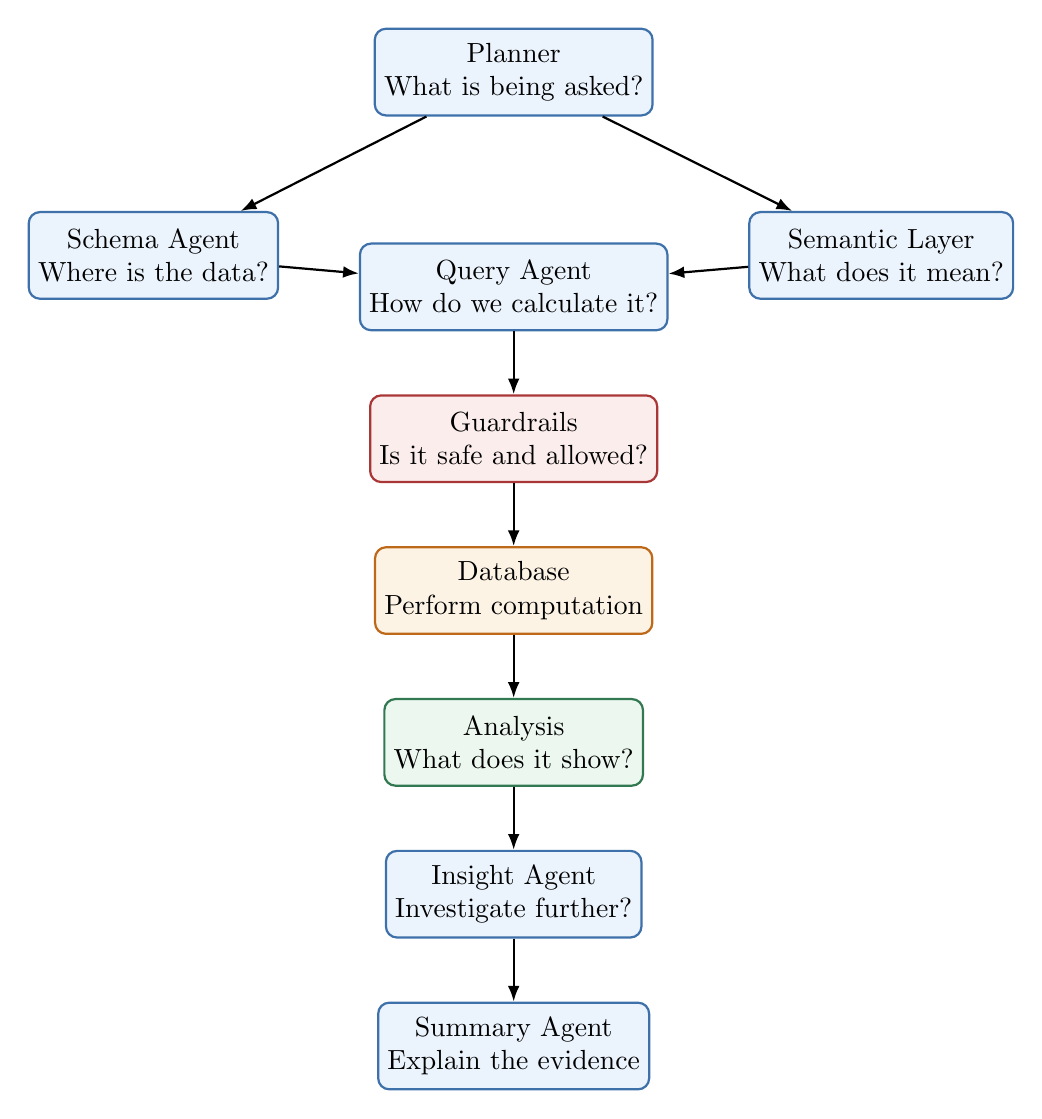
\begin{tikzpicture}[node distance=8mm and 10mm]
\node[agentbox] (p) {Planner\\What is being asked?};
\node[agentbox, below left=12mm and 12mm of p] (s) {Schema Agent\\Where is the data?};
\node[agentbox, below right=12mm and 12mm of p] (m) {Semantic Layer\\What does it mean?};
\node[agentbox, below=16mm of p] (q) {Query Agent\\How do we calculate it?};
\node[securitybox, below=of q] (g) {Guardrails\\Is it safe and allowed?};
\node[databox, below=of g] (d) {Database\\Perform computation};
\node[toolbox, below=of d] (a) {Analysis\\What does it show?};
\node[agentbox, below=of a] (i) {Insight Agent\\Investigate further?};
\node[agentbox, below=of i] (r) {Summary Agent\\Explain the evidence};

\draw[flow] (p)--(s);
\draw[flow] (p)--(m);
\draw[flow] (s)--(q);
\draw[flow] (m)--(q);
\draw[flow] (q)--(g);
\draw[flow] (g)--(d);
\draw[flow] (d)--(a);
\draw[flow] (a)--(i);
\draw[flow] (i)--(r);
\end{tikzpicture}
\caption{Separation of agent responsibilities.}
\label{fig:agents}
\end{figure}

\section{Agentic Investigation Loop}

A fixed Text-to-SQL pipeline answers one question. An agentic analyzer can
continue investigating when an intermediate result suggests a useful
drill-down.

\begin{figure}[H]
\centering
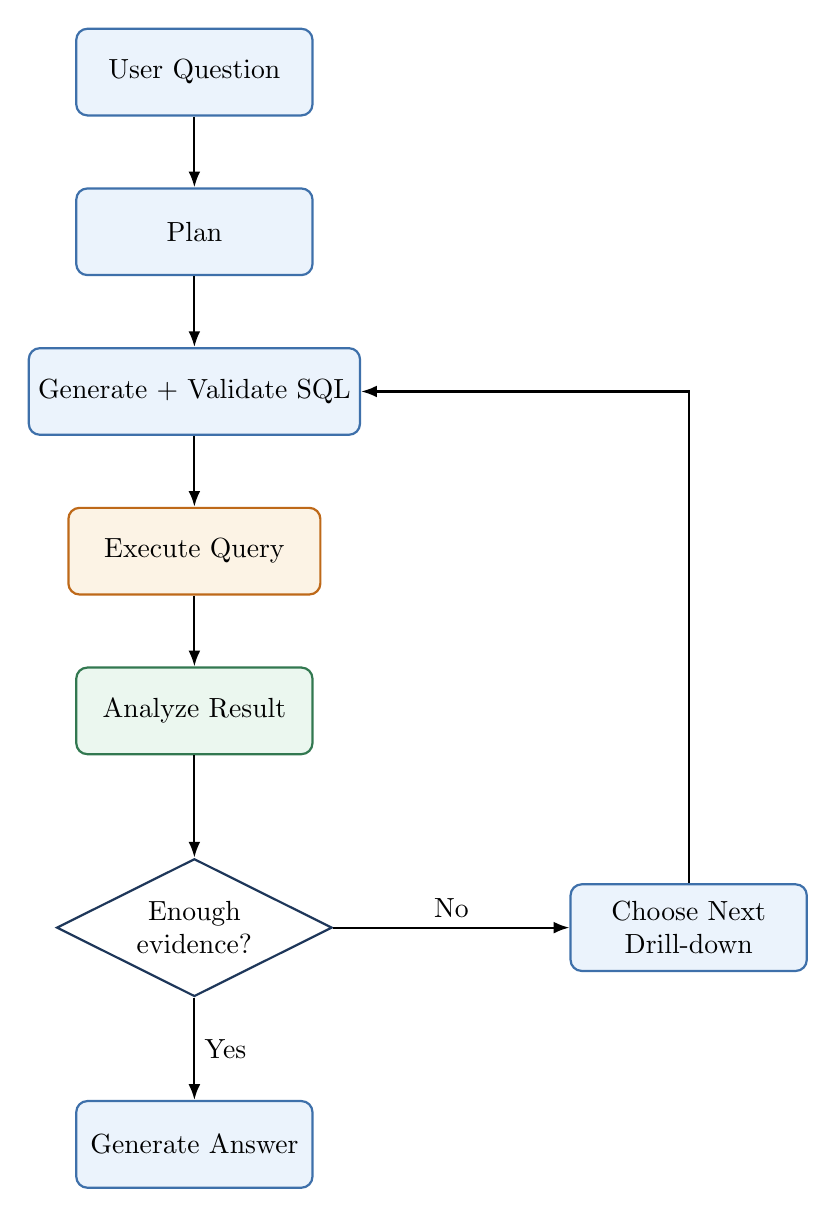
\begin{tikzpicture}[node distance=9mm and 17mm]
\node[agentbox] (q) {User Question};
\node[agentbox, below=of q] (p) {Plan};
\node[agentbox, below=of p] (sql) {Generate + Validate SQL};
\node[databox, below=of sql] (db) {Execute Query};
\node[toolbox, below=of db] (an) {Analyze Result};
\node[decision, below=13mm of an] (dec) {Enough\\evidence?};
\node[agentbox, below=13mm of dec] (ans) {Generate Answer};
\node[agentbox, right=30mm of dec] (drill) {Choose Next\\Drill-down};

\draw[flow] (q)--(p);
\draw[flow] (p)--(sql);
\draw[flow] (sql)--(db);
\draw[flow] (db)--(an);
\draw[flow] (an)--(dec);
\draw[flow] (dec)--node[right]{Yes}(ans);
\draw[flow] (dec)--node[above]{No}(drill);
\draw[flow] (drill)|-(sql);
\end{tikzpicture}
\caption{Bounded agentic investigation loop.}
\label{fig:loop}
\end{figure}

The loop should be bounded by maximum steps, query count, execution time,
estimated cost, and result size.

\section{Schema RAG and Semantic Layer}

For a database containing thousands of tables, the LLM should retrieve only
the relevant metadata.

\begin{figure}[H]
\centering
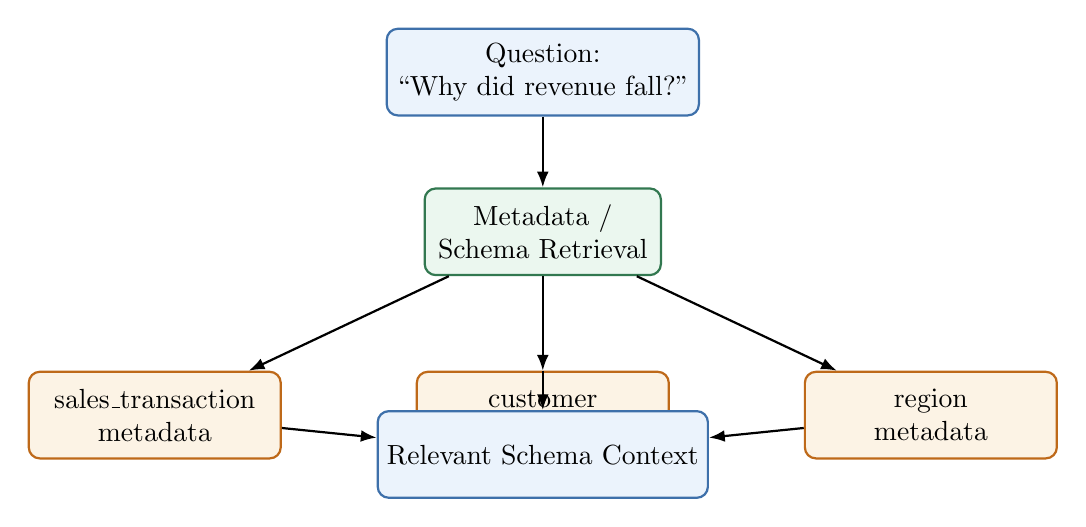
\begin{tikzpicture}[node distance=9mm and 13mm]
\node[agentbox] (question) {Question:\\``Why did revenue fall?''};
\node[toolbox, below=of question] (retrieve) {Metadata /\\Schema Retrieval};
\node[databox, below left=12mm and 18mm of retrieve] (t1)
{sales\_transaction\\metadata};
\node[databox, below=12mm of retrieve] (t2)
{customer\\metadata};
\node[databox, below right=12mm and 18mm of retrieve] (t3)
{region\\metadata};
\node[agentbox, below=17mm of retrieve] (context)
{Relevant Schema Context};

\draw[flow] (question)--(retrieve);
\draw[flow] (retrieve)--(t1);
\draw[flow] (retrieve)--(t2);
\draw[flow] (retrieve)--(t3);
\draw[flow] (t1)--(context);
\draw[flow] (t2)--(context);
\draw[flow] (t3)--(context);
\end{tikzpicture}
\caption{RAG-style retrieval over database metadata.}
\label{fig:schemarag}
\end{figure}

The semantic layer then resolves business concepts such as ``revenue'' into
certified definitions before SQL generation.

\begin{figure}[H]
\centering
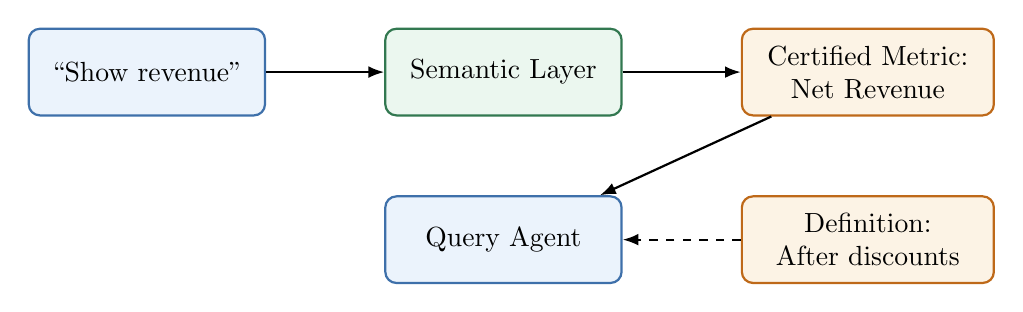
\begin{tikzpicture}[node distance=10mm and 15mm]
\node[agentbox] (q) {``Show revenue''};
\node[toolbox, right=of q] (sem) {Semantic Layer};
\node[databox, right=of sem] (metric) {Certified Metric:\\Net Revenue};
\node[databox, below=of metric] (def) {Definition:\\After discounts};
\node[agentbox, left=of def] (sql) {Query Agent};

\draw[flow] (q)--(sem);
\draw[flow] (sem)--(metric);
\draw[flow] (metric)--(sql);
\draw[dashedflow] (def)--(sql);
\end{tikzpicture}
\caption{Business semantics before SQL generation.}
\label{fig:semanticlayer}
\end{figure}

\section{Safe Text-to-SQL Pipeline}

\begin{figure}[H]
\centering
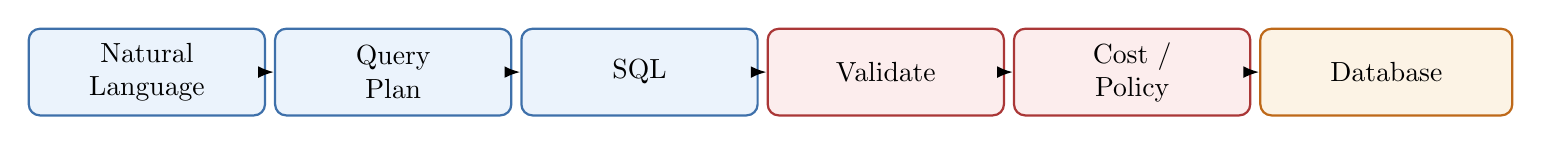
\begin{tikzpicture}[node distance=2mm and 1mm]
\node[agentbox] (nl) {Natural\\Language};
\node[agentbox, right=of nl] (plan) {Query\\Plan};
\node[agentbox, right=of plan] (sql) {SQL};
\node[securitybox, right=of sql] (v) {Validate};
\node[securitybox, right=of v] (c) {Cost /\\Policy};
\node[databox, right=of c] (db) {Database};

\draw[flow] (nl)--(plan);
\draw[flow] (plan)--(sql);
\draw[flow] (sql)--(v);
\draw[flow] (v)--(c);
\draw[flow] (c)--(db);
\end{tikzpicture}
\caption{Controlled Text-to-SQL execution path.}
\label{fig:textsql}
\end{figure}

The validation layer should enforce read-only access, permitted tables and
columns, required filters, join safety, estimated query cost, and timeouts.

\section{Large-Scale Data Flow}

The LLM should not receive billions of raw records.

\begin{figure}[H]
\centering
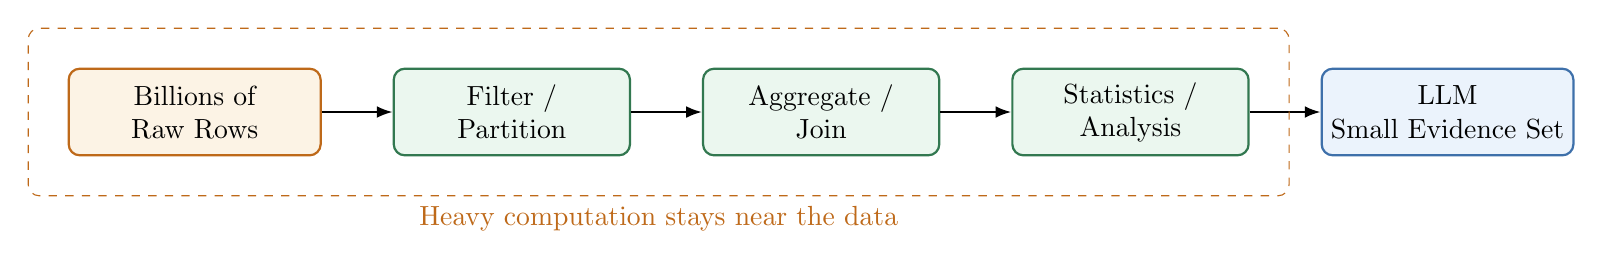
\begin{tikzpicture}[node distance=9mm and 9mm]
\node[databox] (raw) {Billions of\\Raw Rows};
\node[toolbox, right=of raw] (filter) {Filter /\\Partition};
\node[toolbox, right=of filter] (agg) {Aggregate /\\Join};
\node[toolbox, right=of agg] (stats) {Statistics /\\Analysis};
\node[agentbox, right=of stats] (llm) {LLM\\Small Evidence Set};

\draw[flow] (raw)--(filter);
\draw[flow] (filter)--(agg);
\draw[flow] (agg)--(stats);
\draw[flow] (stats)--(llm);

\node[draw=orange2, dashed, rounded corners, fit=(raw)(filter)(agg)(stats),
      inner sep=5mm, label={[orange2]below:Heavy computation stays near the data}] {};
\end{tikzpicture}
\caption{Database-side computation before LLM interpretation.}
\label{fig:scale}
\end{figure}

Useful techniques include partitioning, columnar storage, materialized views,
pre-aggregation, OLAP engines, lakehouses, caching, parallel queries, and
resource quotas.

\section{Hierarchical Summarization}

For extremely large datasets, summaries can be produced at increasing levels
of aggregation.

\begin{figure}[H]
\centering
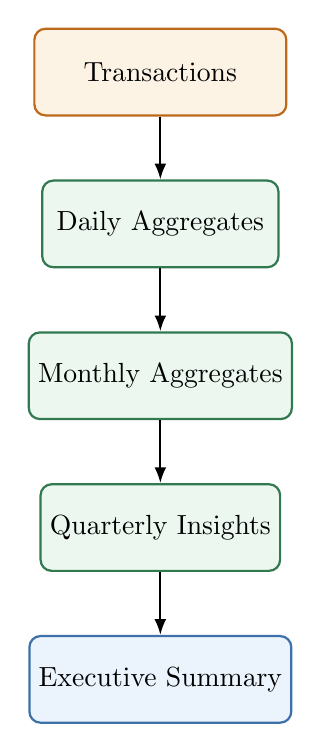
\begin{tikzpicture}[node distance=8mm]
\node[databox] (raw) {Transactions};
\node[toolbox, below=of raw] (daily) {Daily Aggregates};
\node[toolbox, below=of daily] (monthly) {Monthly Aggregates};
\node[toolbox, below=of monthly] (quarterly) {Quarterly Insights};
\node[agentbox, below=of quarterly] (annual) {Executive Summary};

\draw[flow] (raw)--(daily);
\draw[flow] (daily)--(monthly);
\draw[flow] (monthly)--(quarterly);
\draw[flow] (quarterly)--(annual);
\end{tikzpicture}
\caption{Hierarchical summarization.}
\label{fig:hierarchical}
\end{figure}

This resembles a MapReduce pattern: analyze smaller units first, then combine
the resulting summaries.

\section{Evidence and Explainability}

A generated insight should be connected to the evidence that supports it.

\begin{figure}[H]
\centering
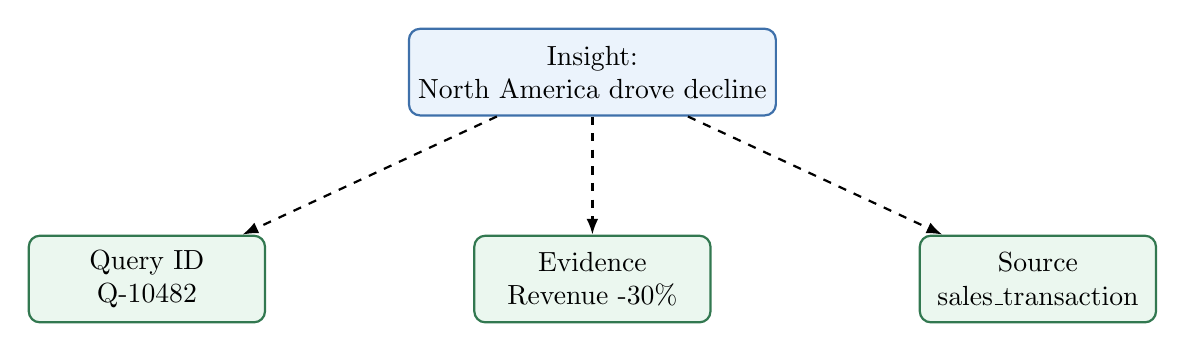
\begin{tikzpicture}[node distance=10mm and 18mm]
\node[agentbox] (insight) {Insight:\\North America drove decline};
\node[toolbox, below left=15mm and 18mm of insight] (queryid)
{Query ID\\Q-10482};
\node[toolbox, below=15mm of insight] (number)
{Evidence\\Revenue -30\%};
\node[toolbox, below right=15mm and 18mm of insight] (source)
{Source\\sales\_transaction};

\draw[dashedflow] (insight)--(queryid);
\draw[dashedflow] (insight)--(number);
\draw[dashedflow] (insight)--(source);
\end{tikzpicture}
\caption{Evidence binding for explainability and auditability.}
\label{fig:evidence}
\end{figure}

This enables query lineage, reproducibility, debugging, audit trails, and
greater user trust.

\section{Security and Governance}

Authorization should not be delegated to the LLM.

\begin{figure}[H]
\centering
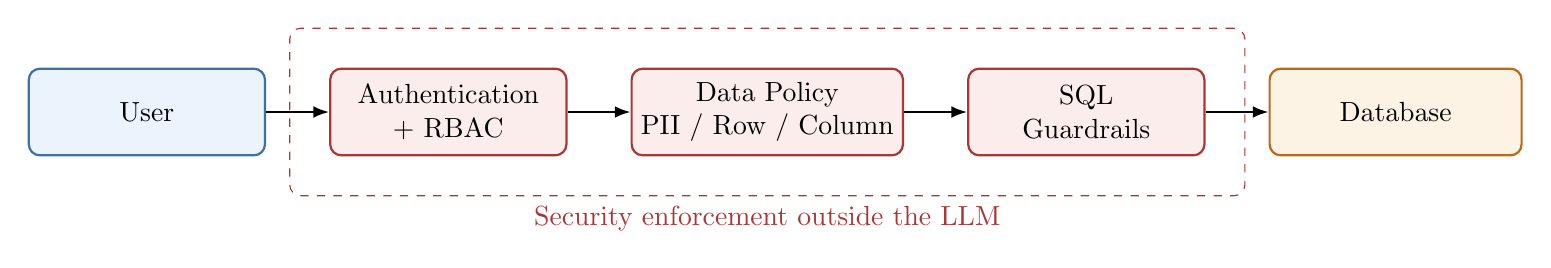
\begin{tikzpicture}[node distance=8mm and 8mm]
\node[agentbox] (user) {User};
\node[securitybox, right=of user] (auth) {Authentication\\+ RBAC};
\node[securitybox, right=of auth] (policy) {Data Policy\\PII / Row / Column};
\node[securitybox, right=of policy] (guard) {SQL\\Guardrails};
\node[databox, right=of guard] (db) {Database};

\draw[flow] (user)--(auth);
\draw[flow] (auth)--(policy);
\draw[flow] (policy)--(guard);
\draw[flow] (guard)--(db);

\node[draw=red2, dashed, rounded corners, fit=(auth)(policy)(guard),
      inner sep=5mm, label={[red2]below:Security enforcement outside the LLM}] {};
\end{tikzpicture}
\caption{Defense-in-depth security controls.}
\label{fig:security}
\end{figure}

\section{End-to-End Example}

For the question ``Why did revenue decline in Q2?'', the system may perform:

\begin{figure}[H]
\centering
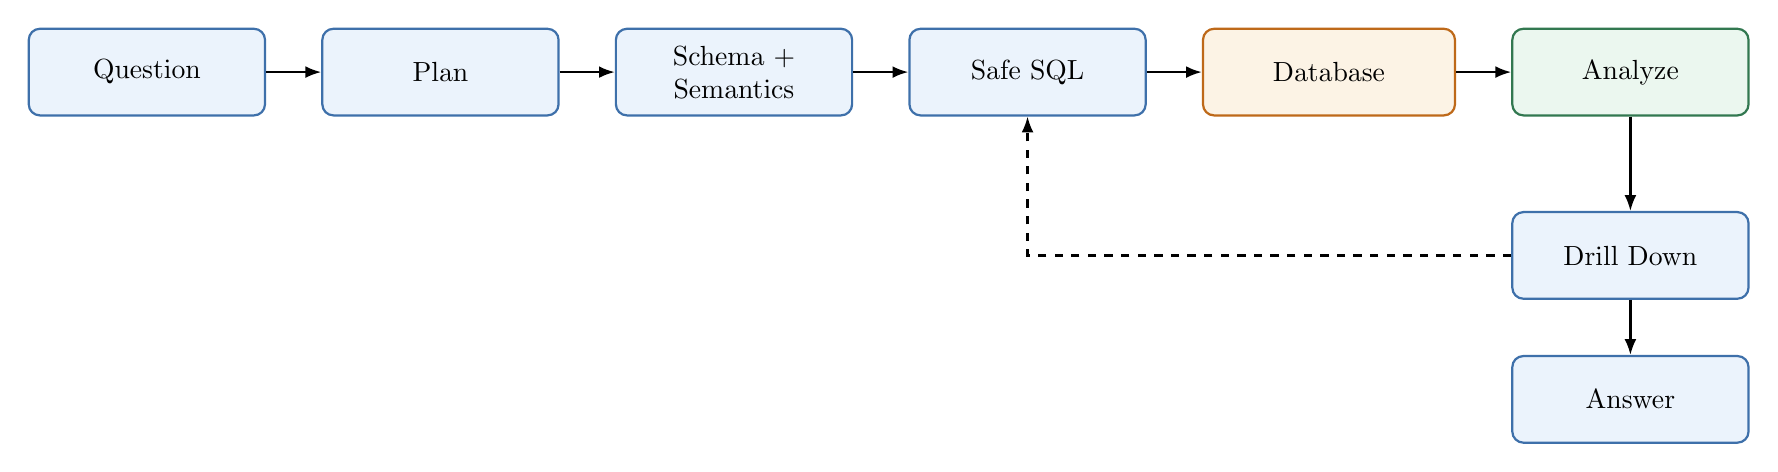
\begin{tikzpicture}[node distance=7mm and 7mm]
\node[agentbox] (q) {Question};
\node[agentbox, right=of q] (p) {Plan};
\node[agentbox, right=of p] (s) {Schema +\\Semantics};
\node[agentbox, right=of s] (sql) {Safe SQL};
\node[databox, right=of sql] (db) {Database};
\node[toolbox, right=of db] (a) {Analyze};
\node[agentbox, below=12mm of a] (i) {Drill Down};
\node[agentbox, below=of i] (r) {Answer};

\draw[flow] (q)--(p);
\draw[flow] (p)--(s);
\draw[flow] (s)--(sql);
\draw[flow] (sql)--(db);
\draw[flow] (db)--(a);
\draw[flow] (a)--(i);
\draw[flow] (i)--(r);
\draw[dashedflow] (i.west) -| (sql.south);
\end{tikzpicture}
\caption{Simplified end-to-end investigation.}
\label{fig:e2e}
\end{figure}

A possible evidence chain is:

\begin{enumerate}
    \item Revenue declined by 12\%.
    \item Region analysis identifies North America as the major contributor.
    \item North America declined by 30\%.
    \item Product analysis identifies Product X as the major contributor.
    \item Product X explains approximately 65\% of the regional decline.
    \item Customer-segment analysis identifies enterprise customers as the
    largest affected segment.
\end{enumerate}

\section{Recommended Student POC Roadmap}

\begin{figure}[H]
\centering
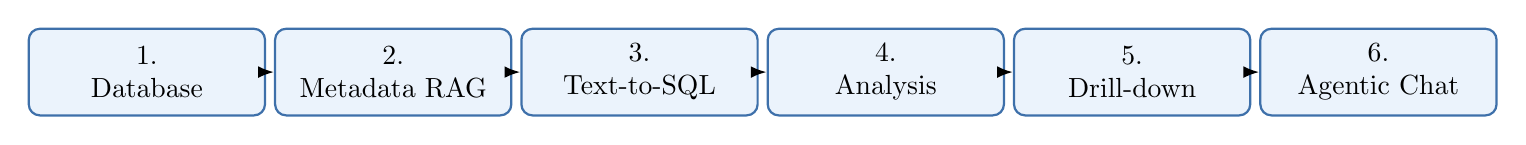
\begin{tikzpicture}[node distance=2mm and 1mm]
\node[agentbox] (p1) {1.\\Database};
\node[agentbox, right=of p1] (p2) {2.\\Metadata RAG};
\node[agentbox, right=of p2] (p3) {3.\\Text-to-SQL};
\node[agentbox, right=of p3] (p4) {4.\\Analysis};
\node[agentbox, right=of p4] (p5) {5.\\Drill-down};
\node[agentbox, right=of p5] (p6) {6.\\Agentic Chat};

\draw[flow] (p1)--(p2);
\draw[flow] (p2)--(p3);
\draw[flow] (p3)--(p4);
\draw[flow] (p4)--(p5);
\draw[flow] (p5)--(p6);
\end{tikzpicture}
\caption{Incremental POC roadmap.}
\label{fig:roadmap}
\end{figure}

\section{Design Principles}

\begin{enumerate}[leftmargin=*]
    \item LLM as planner and interpreter, not the database engine.
    \item Push computation to the data platform.
    \item Retrieve relevant schema instead of exposing all tables.
    \item Use a semantic layer for business meaning.
    \item Validate SQL before execution.
    \item Use deterministic tools for numerical calculations.
    \item Bound agentic loops with explicit budgets.
    \item Keep authorization outside the LLM.
    \item Record evidence and lineage.
    \item Return conclusions with supporting evidence.
    \item Start with a controlled POC before introducing full autonomy.
\end{enumerate}

\section{Discussion Questions}

\begin{enumerate}
    \item What changes if the database contains 10 billion rows?
    \item How can the agent find the right table among 10,000 tables?
    \item How should ``revenue'' be resolved when multiple definitions exist?
    \item How can expensive full-table scans be prevented?
    \item Should an agent ever execute arbitrary SQL?
    \item How should PII and row-level access be protected?
    \item What happens when two agents produce contradictory findings?
    \item How should SQL accuracy and answer faithfulness be evaluated?
    \item When should an autonomous investigation stop?
    \item Which operations should be deterministic rather than LLM-generated?
\end{enumerate}

\section{Key Takeaway}

\[
\boxed{\text{Database} \rightarrow \text{LLM} \rightarrow \text{Summary}}
\]

is a poor architecture for large-scale data analysis.

A more robust architecture is:

\[
\boxed{
\text{User}
\rightarrow
\text{Planner}
\rightarrow
\text{Metadata / Semantics}
\rightarrow
\text{Safe Query}
\rightarrow
\text{Database}
\rightarrow
\text{Analysis}
\rightarrow
\text{Evidence}
\rightarrow
\text{LLM Summary}
}
\]

\begin{center}
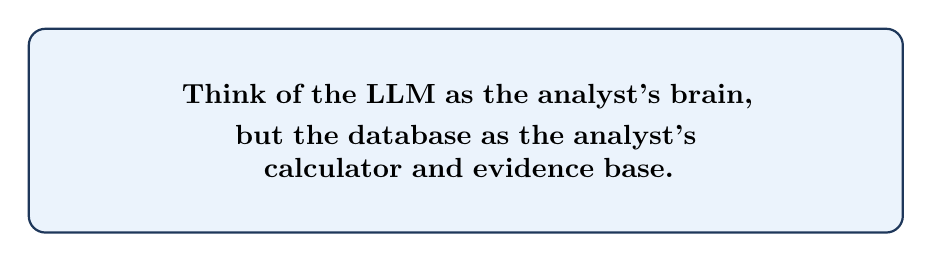
\begin{tikzpicture}
\node[draw=navy, rounded corners=6pt, thick, fill=lightblue,
      text width=0.80\textwidth, align=center, inner sep=7mm] {
\textbf{Think of the LLM as the analyst's brain,}\\[1mm]
\textbf{but the database as the analyst's calculator and evidence base.}
};
\end{tikzpicture}
\end{center}

\tableofcontents
\newpage

\section{Problem Statement}

Consider an organization with a large analytical database containing
customers, orders, products, transactions, regions, support interactions, and
other operational data.

A user may ask:

\begin{quote}
``Summarize our business performance last quarter. Why did revenue decline,
and which products and customer segments caused the decline?''
\end{quote}

A conventional chatbot cannot simply retrieve every row and send it to an
LLM. The database may contain millions or billions of rows.

The desired system therefore needs to behave more like an intelligent
analyst:

\begin{enumerate}[leftmargin=*]
    \item Understand the user's question.
    \item Identify the relevant business concepts and metrics.
    \item Discover the relevant database schema.
    \item Formulate an analytical plan.
    \item Generate safe and efficient database queries.
    \item Execute computation close to the data.
    \item Inspect the results.
    \item Decide whether additional investigation is required.
    \item Produce a concise, evidence-based explanation.
    \item Support follow-up questions while preserving conversation context.
\end{enumerate}

The key architectural idea is:

\begin{quote}
\important{The agent should not read the database; the agent should decide
what the database needs to calculate.}
\end{quote}

\section{System Goals}

The proposed system should provide:

\begin{itemize}[leftmargin=*]
    \item Natural-language access to structured data.
    \item Safe Text-to-SQL generation.
    \item Metadata-aware schema discovery.
    \item Business-semantic understanding of metrics.
    \item Scalable analysis of very large datasets.
    \item Multi-step investigative reasoning.
    \item Conversational follow-up.
    \item Query and reasoning traceability.
    \item Access control and data protection.
    \item Clear separation between computation and language generation.
\end{itemize}

\section{High-Level Architecture}

Figure~\ref{fig:architecture} shows the conceptual architecture.

\begin{figure}[ht]
\centering
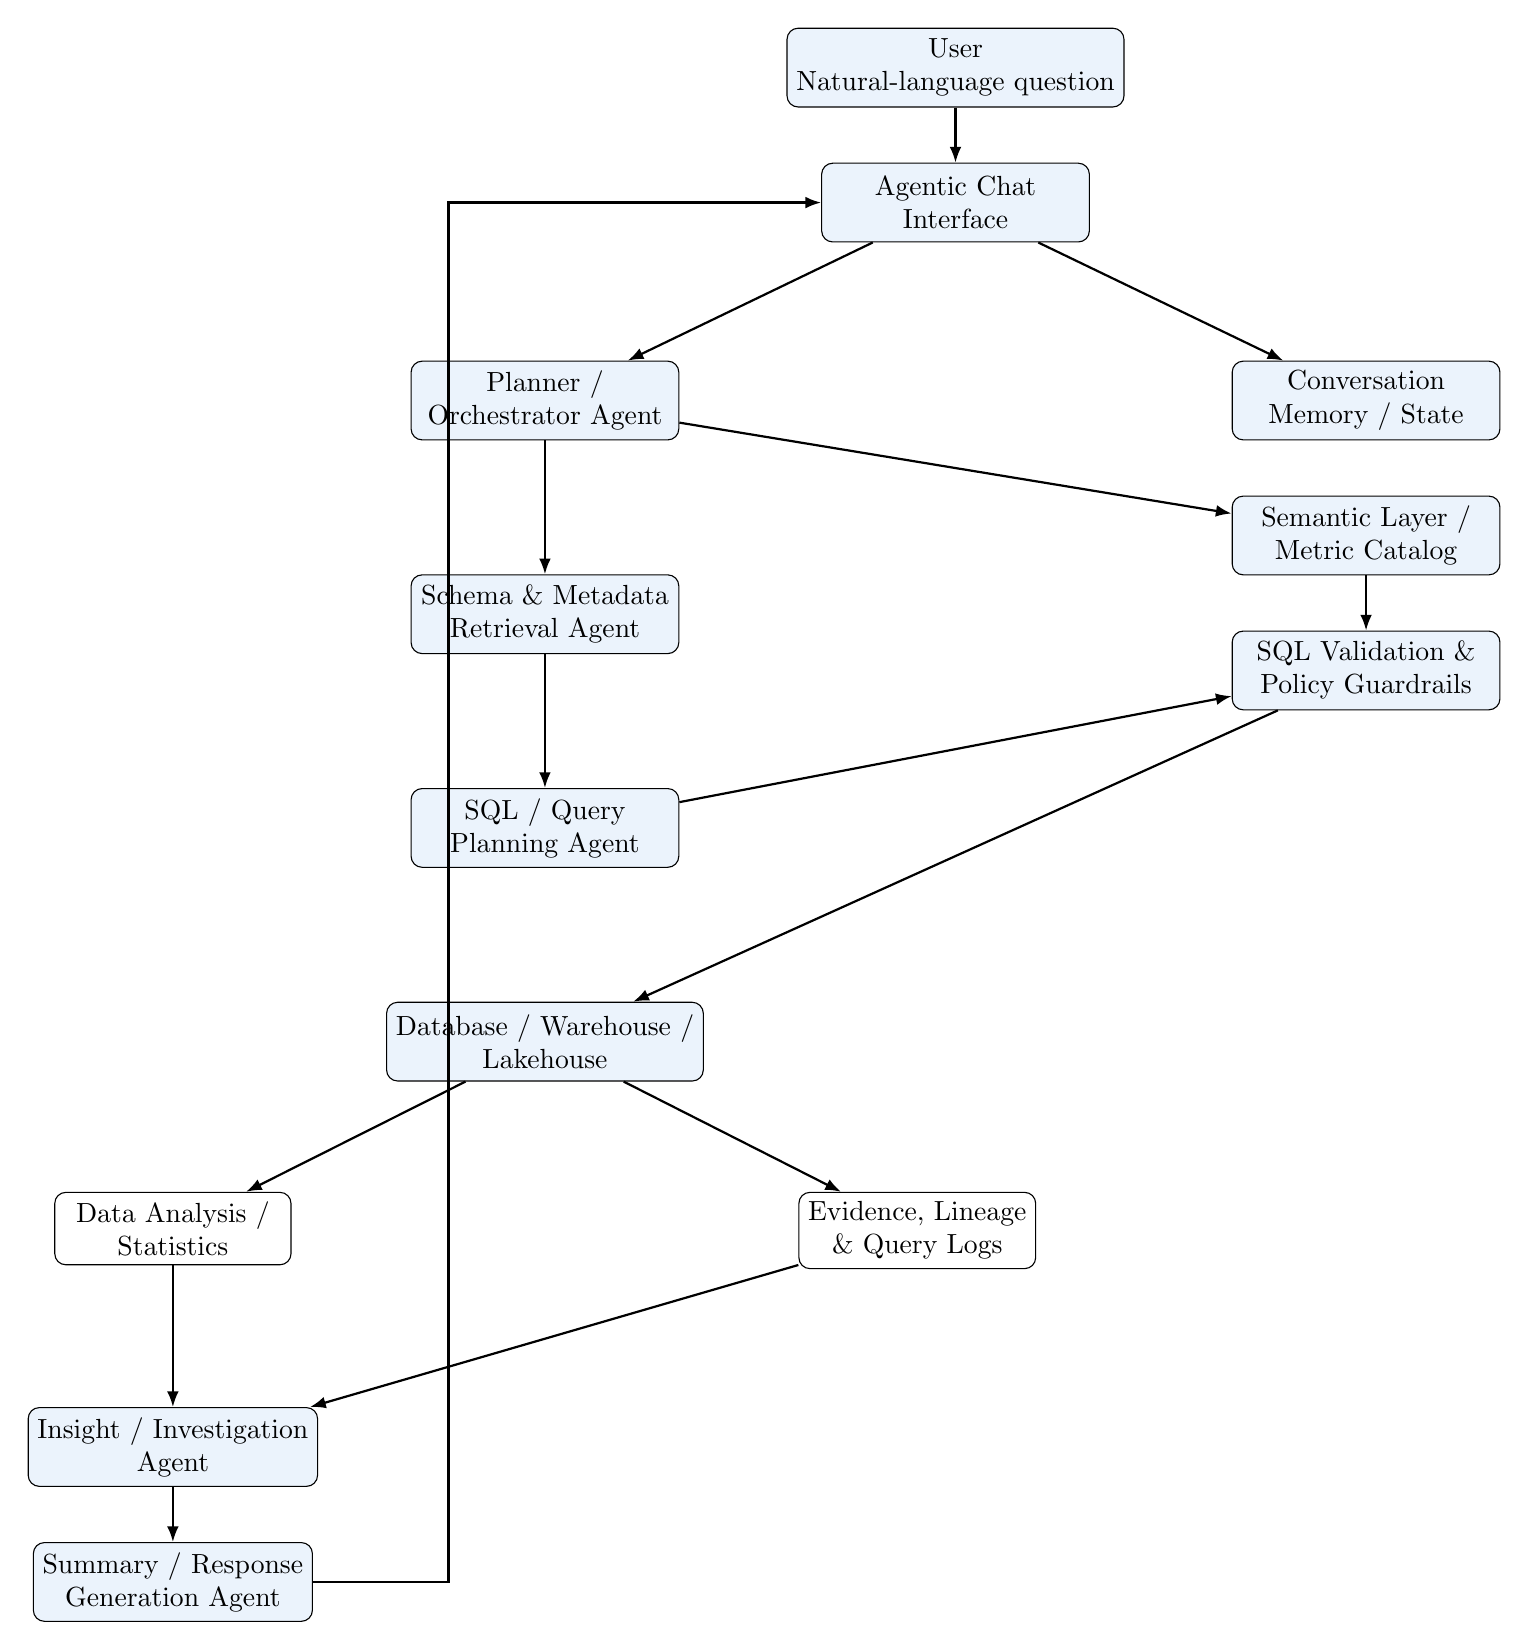
\begin{tikzpicture}[
    node distance=7mm and 12mm,
    box/.style={draw, rounded corners, align=center, minimum width=34mm,
                minimum height=10mm, fill=lightblue},
    smallbox/.style={draw, rounded corners, align=center, minimum width=30mm,
                minimum height=9mm, fill=white},
    arrow/.style={-{Latex[length=2mm]}, thick}
]

\node[box] (user) {User\\Natural-language question};
\node[box, below=of user] (chat) {Agentic Chat\\Interface};

\node[box, below left=15mm and 18mm of chat] (planner)
    {Planner /\\Orchestrator Agent};
\node[box, below right=15mm and 18mm of chat] (memory)
    {Conversation\\Memory / State};

\node[box, below=17mm of planner] (schema)
    {Schema \& Metadata\\Retrieval Agent};
\node[box, below=of memory] (semantic)
    {Semantic Layer /\\Metric Catalog};

\node[box, below=17mm of schema] (sql)
    {SQL / Query\\Planning Agent};
\node[box, below=of semantic] (guard)
    {SQL Validation \&\\Policy Guardrails};

\node[box, below=17mm of sql] (db)
    {Database / Warehouse /\\Lakehouse};

\node[smallbox, below left=14mm and 12mm of db] (analysis)
    {Data Analysis /\\Statistics};
\node[smallbox, below right=14mm and 12mm of db] (evidence)
    {Evidence, Lineage\\\& Query Logs};

\node[box, below=18mm of analysis] (insight)
    {Insight / Investigation\\Agent};

\node[box, below=of insight] (summary)
    {Summary / Response\\Generation Agent};

\draw[arrow] (user) -- (chat);
\draw[arrow] (chat) -- (planner);
\draw[arrow] (chat) -- (memory);
\draw[arrow] (planner) -- (schema);
\draw[arrow] (planner) -- (semantic);
\draw[arrow] (schema) -- (sql);
\draw[arrow] (semantic) -- (guard);
\draw[arrow] (sql) -- (guard);
\draw[arrow] (guard) -- (db);
\draw[arrow] (db) -- (analysis);
\draw[arrow] (db) -- (evidence);
\draw[arrow] (analysis) -- (insight);
\draw[arrow] (evidence) -- (insight);
\draw[arrow] (insight) -- (summary);
\draw[arrow] (summary) -- ++(35mm,0) |- (chat);

\end{tikzpicture}
\caption{Conceptual architecture of the multi-agent Database Analyzer.}
\label{fig:architecture}
\end{figure}

\section{Why a Multi-Agent Architecture?}

A single LLM prompt can perform simple Text-to-SQL tasks, but a production
system needs several distinct responsibilities.

For example:

\begin{longtable}{p{0.23\textwidth} p{0.68\textwidth}}
\toprule
\textbf{Component} & \textbf{Primary responsibility}\\
\midrule
Planner & Converts the user request into an analytical plan.\\
Schema Agent & Finds relevant tables, columns, relationships, and metadata.\\
Semantic Layer & Resolves business meanings such as ``revenue'' or ``active customer''.\\
Query Agent & Generates analytical SQL or query plans.\\
Guardrail Agent & Validates SQL, permissions, cost, and safety constraints.\\
Analysis Agent & Computes trends, comparisons, anomalies, and statistical findings.\\
Insight Agent & Decides whether additional drill-down is necessary.\\
Summary Agent & Converts evidence into a readable explanation.\\
Memory & Maintains conversational context and prior analytical state.\\
\bottomrule
\end{longtable}

These components do not necessarily need to be separate LLM instances.
They are logical responsibilities that can initially be implemented using a
single orchestrator and progressively separated as the system grows.

\section{Agentic Chat Support}

The chat interface is more than a Text-to-SQL interface.

Suppose the user asks:

\begin{quote}
``What happened to revenue last quarter?''
\end{quote}

The system might first discover:

\begin{enumerate}
    \item Revenue decreased by 12\%.
    \item North America contributed most of the decline.
    \item Product X explains most of the North American decline.
    \item Enterprise customers experienced the largest reduction.
\end{enumerate}

The user can then ask:

\begin{quote}
``Why did Product X decline?''
\end{quote}

The system should not start from scratch. It should retain analytical state
and understand that ``Product X'' refers to the previously identified product.

A useful conversation state can include:

\begin{lstlisting}
{
  "time_period": "previous quarter",
  "metric": "net_revenue",
  "analysis_context": "revenue_decline",
  "identified_region": "North America",
  "identified_product": "Product X",
  "previous_queries": [...],
  "evidence": [...]
}
\end{lstlisting}

This enables conversational investigation.

\section{Agentic Investigation Loop}

The key difference between a fixed pipeline and an agentic system is the
ability to decide whether more analysis is needed.

\begin{figure}[ht]
\centering
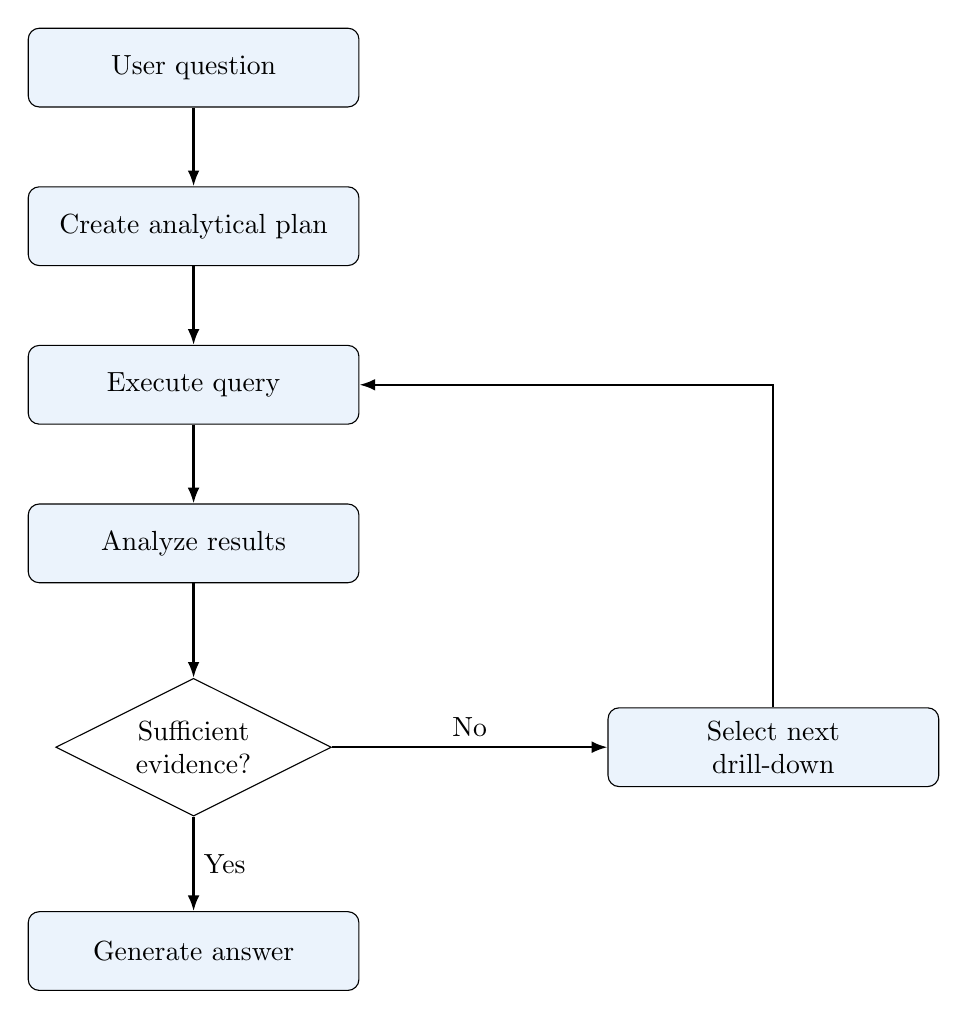
\begin{tikzpicture}[
    node distance=10mm and 20mm,
    box/.style={draw, rounded corners, align=center, minimum width=42mm,
                minimum height=10mm, fill=lightblue},
    decision/.style={diamond, draw, aspect=2, align=center, fill=white},
    arrow/.style={-{Latex[length=2mm]}, thick}
]
\node[box] (q) {User question};
\node[box, below=of q] (plan) {Create analytical plan};
\node[box, below=of plan] (query) {Execute query};
\node[box, below=of query] (analyze) {Analyze results};
\node[decision, below=12mm of analyze] (enough) {Sufficient\\evidence?};
\node[box, below=12mm of enough] (summary) {Generate answer};
\node[box, right=35mm of enough] (drill) {Select next\\drill-down};

\draw[arrow] (q)--(plan);
\draw[arrow] (plan)--(query);
\draw[arrow] (query)--(analyze);
\draw[arrow] (analyze)--(enough);
\draw[arrow] (enough)--node[right]{Yes}(summary);
\draw[arrow] (enough)--node[above]{No}(drill);
\draw[arrow] (drill)|-(query);
\end{tikzpicture}
\caption{Agentic investigation loop.}
\end{figure}

The loop must be bounded. Otherwise, an autonomous agent can generate
unnecessary queries and consume significant database resources.

Useful controls include:

\begin{itemize}
    \item Maximum number of reasoning steps.
    \item Maximum number of database queries.
    \item Query timeout.
    \item Maximum estimated query cost.
    \item Maximum rows returned to the LLM.
    \item Allowed tables and columns.
    \item User-specific access policies.
\end{itemize}

\section{Schema and Metadata Design}

Schema discovery is one of the most important components of the system.

A large enterprise database may contain thousands of tables. Supplying the
entire schema to an LLM is inefficient.

Instead, maintain a metadata catalog.

A useful metadata record might contain:

\begin{lstlisting}
{
  "table": "sales_transaction",
  "description": "Completed customer sales transactions",
  "business_domain": "Sales",
  "owner": "Finance",
  "certified": true,
  "columns": [
    {
      "name": "transaction_date",
      "description": "Date of completed transaction",
      "semantic_type": "date"
    },
    {
      "name": "customer_id",
      "description": "Unique customer identifier",
      "semantic_type": "identifier"
    },
    {
      "name": "net_revenue",
      "description": "Revenue after discounts",
      "semantic_type": "currency"
    }
  ]
}
\end{lstlisting}

The schema metadata can be indexed for semantic retrieval.

For example:

\[
\text{User Question}
\rightarrow
\text{Metadata Retrieval}
\rightarrow
\text{Relevant Tables}
\rightarrow
\text{Relevant Columns}
\]

This is effectively \textbf{RAG over database metadata}.

\section{Semantic Layer and Business Metrics}

Technical schema alone is not enough.

Consider the word ``revenue''. It may refer to:

\begin{itemize}
    \item Gross revenue.
    \item Net revenue.
    \item Recognized revenue.
    \item Booked revenue.
    \item Recurring revenue.
    \item Cash collected.
\end{itemize}

A semantic layer can define the organization's approved business metrics.

For example:

\begin{lstlisting}
Metric: Net Revenue

Definition:
Revenue recognized after discounts and adjustments.

Formula:
SUM(net_revenue)

Source:
finance_revenue

Owner:
Finance

Certified:
Yes
\end{lstlisting}

This significantly reduces the risk that the LLM generates technically valid
but business-incorrect SQL.

\section{Query Generation and Validation}

The Query Agent should not be allowed to execute arbitrary SQL.

A recommended pipeline is:

\[
\text{Natural Language}
\rightarrow
\text{Query Plan}
\rightarrow
\text{SQL}
\rightarrow
\text{Validation}
\rightarrow
\text{Cost Check}
\rightarrow
\text{Execution}
\]

Validation should check:

\begin{itemize}
    \item SQL syntax.
    \item Allowed tables.
    \item Allowed columns.
    \item User permissions.
    \item Prohibited operations.
    \item Missing filters.
    \item Cartesian joins.
    \item Excessive scan risk.
    \item Query timeout.
    \item Estimated cost.
\end{itemize}

For analytical workloads, read-only database credentials should normally be
used by the agent.

\section{Scaling to Very Large Databases}

The most important scaling principle is:

\begin{quote}
\important{Move computation to the data rather than moving the data to the
LLM.}
\end{quote}

The system should avoid:

\begin{lstlisting}
SELECT * FROM billion_row_table;
\end{lstlisting}

Instead, it should push computation into the database:

\begin{lstlisting}
SELECT
    region,
    SUM(net_revenue) AS revenue,
    COUNT(DISTINCT customer_id) AS customers
FROM sales_transaction
WHERE transaction_date >= DATE '2026-04-01'
  AND transaction_date <  DATE '2026-07-01'
GROUP BY region;
\end{lstlisting}

The LLM receives the small aggregated result rather than the raw records.

\subsection{Scaling Techniques}

Important techniques include:

\begin{itemize}
    \item Partitioning by time or business dimensions.
    \item Indexing where appropriate.
    \item Columnar storage.
    \item Materialized views.
    \item Pre-aggregated fact tables.
    \item OLAP warehouses.
    \item Data lakehouse architectures.
    \item Query result caching.
    \item Approximate algorithms for expensive distinct counts.
    \item Parallel analytical queries.
    \item Workload management and resource quotas.
\end{itemize}

\section{Hierarchical Summarization}

For very large datasets, analysis can be hierarchical.

For example:

\[
\text{Transaction Data}
\rightarrow
\text{Daily Aggregates}
\rightarrow
\text{Monthly Aggregates}
\rightarrow
\text{Quarterly Insights}
\rightarrow
\text{Annual Summary}
\]

This resembles a MapReduce pattern:

\[
\text{Map: Analyze smaller units}
\]

\[
\text{Reduce: Combine the resulting summaries}
\]

The LLM should generally operate on the smaller, higher-level analytical
representation.

\section{Data Analysis and Insight Detection}

The Data Analysis Agent can perform deterministic calculations before the
LLM sees the data.

Examples include:

\begin{itemize}
    \item Percentage change.
    \item Moving averages.
    \item Trend detection.
    \item Variance analysis.
    \item Outlier detection.
    \item Correlation analysis.
    \item Distribution analysis.
    \item Segment comparisons.
\end{itemize}

For example, if quarterly revenue changes from \(120M\) to \(138M\):

\[
Growth =
\frac{138-120}{120}\times100
=15\%
\]

The LLM should not be responsible for doing every numerical calculation
itself. Deterministic tools should calculate the numbers; the LLM should
interpret them.

\section{Evidence and Explainability}

Every generated insight should ideally have supporting evidence.

A response could maintain:

\begin{lstlisting}
Insight:
North America caused most of the revenue decline.

Evidence:
Query ID: Q-10482
Revenue change: -30%
Contribution to total decline: 72%

Source tables:
sales_transaction
customer
region
\end{lstlisting}

This provides a foundation for:

\begin{itemize}
    \item Auditability.
    \item Debugging.
    \item User trust.
    \item Reproducibility.
    \item Governance.
\end{itemize}

The final answer should distinguish between:

\begin{enumerate}
    \item Observed facts.
    \item Statistical findings.
    \item Agent-generated interpretations.
    \item Hypotheses requiring further investigation.
\end{enumerate}

\section{Security and Governance}

A database agent is potentially a high-risk system because it can provide
access to sensitive enterprise data.

Security must therefore be enforced outside the LLM.

Important controls include:

\begin{itemize}
    \item Authentication.
    \item Role-based access control (RBAC).
    \item Row-level security.
    \item Column-level security.
    \item PII masking.
    \item Data classification.
    \item Read-only credentials.
    \item Query allowlists and denylists.
    \item Query logging.
    \item Audit trails.
    \item Rate limits.
    \item Cost limits.
\end{itemize}

A critical principle is:

\begin{quote}
\important{Never rely on the LLM to enforce authorization.}
\end{quote}

The database and policy enforcement layers must independently enforce
access restrictions.

\section{Major System Bottlenecks}

\begin{longtable}{p{0.20\textwidth} p{0.32\textwidth} p{0.38\textwidth}}
\toprule
\textbf{Bottleneck} & \textbf{Why it matters} & \textbf{Possible solution}\\
\midrule
Context size & Entire database cannot fit into LLM context. & Aggregation, metadata RAG, hierarchical summarization.\\
Query cost & Poor SQL can scan huge datasets. & Query validation, partitioning, cost estimation, materialized views.\\
Schema complexity & Thousands of tables confuse the model. & Metadata catalog and semantic retrieval.\\
Business semantics & Correct SQL can still answer the wrong business question. & Certified metric definitions and semantic layer.\\
Latency & Multi-step agent loops can be slow. & Parallel queries, caching, pre-aggregation.\\
Security & Database may contain sensitive information. & RBAC, masking, row/column security.\\
Hallucination & LLM may generate invalid SQL or unsupported claims. & SQL validation, evidence binding, deterministic calculations.\\
Agent loops & Autonomous investigation can become expensive. & Step budgets and query budgets.\\
Trust & Users need to know why a conclusion was reached. & Query lineage and evidence references.\\
\bottomrule
\end{longtable}

\section{Recommended Proof-of-Concept}

A practical student POC should start small.

\subsection{Phase 1: Fixed Analytical Database}

Use a database containing tables such as:

\begin{lstlisting}
customers
products
orders
order_items
regions
\end{lstlisting}

Populate it with synthetic data.

\subsection{Phase 2: Metadata Retrieval}

Create metadata describing:

\begin{itemize}
    \item Tables.
    \item Columns.
    \item Relationships.
    \item Business definitions.
\end{itemize}

Add semantic retrieval for schema discovery.

\subsection{Phase 3: Text-to-SQL}

Implement:

\[
\text{Question}
\rightarrow
\text{Relevant Schema}
\rightarrow
\text{SQL}
\]

Add SQL validation before execution.

\subsection{Phase 4: Analysis Agent}

Allow the agent to compare:

\begin{itemize}
    \item Current period vs previous period.
    \item Regions.
    \item Products.
    \item Customer segments.
\end{itemize}

\subsection{Phase 5: Agentic Drill-Down}

Introduce the loop:

\[
\text{Analyze}
\rightarrow
\text{Detect Significant Finding}
\rightarrow
\text{Drill Down}
\rightarrow
\text{Analyze Again}
\]

The loop should stop when sufficient evidence has been collected.

\subsection{Phase 6: Agentic Chat}

Add conversational follow-up:

\begin{quote}
User: ``Summarize Q2 revenue.''

Agent: ``Revenue increased 15\%.''

User: ``Why?''

Agent: ``APAC and Product X were the largest contributors.''

User: ``Tell me more about Product X.''

Agent: ``Product X grew 28\%, mainly among enterprise customers.''
\end{quote}

The conversation state should preserve the analytical context.

\section{Example End-to-End Workflow}

Consider:

\begin{quote}
``Why did revenue decline in Q2?''
\end{quote}

The workflow may be:

\begin{enumerate}
    \item Planner identifies the metric, period, and comparison period.
    \item Schema Agent retrieves revenue and transaction metadata.
    \item Semantic Layer resolves ``revenue'' to the certified metric.
    \item Query Agent creates the initial aggregate query.
    \item Guardrail validates the query.
    \item Database executes the query.
    \item Analysis Agent detects a 12\% decline.
    \item Insight Agent chooses region as the next dimension.
    \item Database calculates regional changes.
    \item North America shows a 30\% decline.
    \item Insight Agent drills into product.
    \item Product X explains most of the decline.
    \item Insight Agent drills into customer segment.
    \item Enterprise customers are identified as the major contributor.
    \item Summary Agent produces the final evidence-based response.
\end{enumerate}

The resulting explanation could be:

\begin{quote}
Revenue declined 12\% in Q2 compared with Q1. The primary driver was a
30\% decline in North America, which accounted for most of the overall
reduction. Product X contributed approximately 65\% of the North American
decline, with enterprise customers representing the largest affected segment.
\end{quote}

The important distinction is that the answer is generated from a chain of
database-backed evidence rather than from the LLM's general knowledge.

\section{Design Principles}

The following principles should guide implementation.

\begin{enumerate}
    \item \textbf{LLM as planner, not database engine.}
    \item \textbf{Push computation to the database.}
    \item \textbf{Retrieve relevant schema rather than exposing everything.}
    \item \textbf{Use a semantic layer for business meaning.}
    \item \textbf{Validate generated SQL before execution.}
    \item \textbf{Use deterministic tools for numerical calculations.}
    \item \textbf{Bound agentic loops.}
    \item \textbf{Keep authorization outside the LLM.}
    \item \textbf{Record evidence and lineage.}
    \item \textbf{Return conclusions with supporting evidence.}
    \item \textbf{Start with a controlled POC before introducing full autonomy.}
\end{enumerate}

\section{Discussion Questions}

Students should consider the following questions when designing their own
implementation:

\begin{enumerate}
    \item What happens if the database contains 10 billion rows?
    \item How can the agent discover the correct table among 10,000 tables?
    \item How should the system resolve an ambiguous term such as ``revenue''?
    \item How can we prevent the agent from generating an expensive full-table scan?
    \item Should the agent be allowed to execute arbitrary SQL?
    \item How should PII be protected?
    \item How should different users receive different database views?
    \item What happens when two agents produce contradictory findings?
    \item How do we evaluate whether the generated SQL is correct?
    \item How do we evaluate whether the final explanation is faithful to the data?
    \item When should the agent stop investigating?
    \item Which operations should be deterministic rather than LLM-generated?
    \item How can query lineage be exposed to the user?
    \item What should be cached?
    \item When does a multi-agent design become unnecessarily complex?
\end{enumerate}

\section{Key Takeaway}

A scalable database-analysis agent is not:

\[
\boxed{\text{Database} \rightarrow \text{LLM} \rightarrow \text{Summary}}
\]

A more robust architecture is:

\[
\boxed{
\text{User}
\rightarrow
\text{Planner}
\rightarrow
\text{Metadata/Semantics}
\rightarrow
\text{Query}
\rightarrow
\text{Database}
\rightarrow
\text{Analysis}
\rightarrow
\text{Evidence}
\rightarrow
\text{LLM Summary}
}
\]

For very large databases, the most important engineering principle is to keep
large-scale computation inside the data platform and provide the LLM with
small, relevant, validated, and explainable results.

The ``agentic'' capability is then used for deciding \emph{what to investigate
next}, rather than for indiscriminately reading data.

\end{document}
